\documentclass[10pt, titlepage]{article}

\usepackage[margin=1in]{geometry}
\usepackage{fancyhdr}
\usepackage{amsfonts}
\usepackage{amsmath}
\usepackage{amssymb}
\usepackage{booktabs}
\usepackage{tikz}
\usepackage{float}
\usepackage{bm}
\usepackage{pgfplots}


\makeatletter
\setlength{\@fptop}{0pt}
\makeatother

\title{\normalsize PLUS Session Worksheet \\[1em] \Large \textit{MATH 1554:} Linear Algebra}
\author{Covering lessons: 6.1 -- 6.2}
\date{Fall 2023}

% ------- Set up header -------
\renewcommand{\sectionmark}[1]{\markright{#1}} % from https://tex.stackexchange.com/a/317393/227665
\pagestyle{fancy}
\fancyhead[L]{Fall 2023}
\fancyhead[C]{\textit{(6.1) \& (6.2)}}
\fancyhead[R]{\textbf{\thepage}}
% -------------------------------------------------------

% ------- Set up Main Idea box environment -------
\newcounter{mainideas}
\setcounter{mainideas}{1}
\newcommand{\mainidea}{\textbf{Main Idea \#\themainideas \stepcounter{mainideas}}}
\setlength\fboxsep{1em}
%\newcommand{\midea}[2]{\begin{center}\fbox{\parbox{#1}{\centering \mainidea #2}} \end{center}} % Could be environment but I couldn't bother

% The way this works is that the savebox collects whatever was between the minipage and the end of it, then in the last line of the definition of the environment
% we regurgigate whatever was collected into an fbox which we center.
\newsavebox{\mybox}
\newenvironment{mideea}[1]
{%
\begin{lrbox}{\mybox}%
	\begin{minipage}{#1\textwidth}
		{\centering \mainidea \par}

}
{\end{minipage}\end{lrbox}\begin{center}\fbox{\usebox{\mybox}}\end{center}}
% -------------------------------------------------------

% ------- Set up activity environment -------
\newcounter{question}
\setcounter{question}{1}
\newenvironment{newquestion}
{
	\noindent\textbf{Question \thequestion}
}
{
\stepcounter{question}
\par
}
% -------------------------------------------------------


% ------- Set up math stuff -------
\renewcommand{\vec}[1]{\bm{#1}}
\DeclareMathOperator{\vspan}{Span}
\DeclareMathOperator{\row}{row}
\DeclareMathOperator{\col}{col}
\DeclareMathOperator{\colspace}{Col}
\DeclareMathOperator{\nullspace}{Nul}
\DeclareMathOperator{\rowspace}{Row}
\DeclareMathOperator{\rank}{rank}
\DeclareMathOperator{\proj}{proj}
% -------------------------------------------------------

% ------- Set up circle -------
\newcommand{\bubble}{\tikz[baseline=-0.625ex]\draw[radius=0.5em, fill=white] (0,0) circle;}
\newcommand{\dbubble}{\tikz[baseline=-0.625ex]\draw[radius=0.5em, fill=black] (0,0) circle;}
% -------------------------------------------------------

\begin{document}
\maketitle

\section{\centering Dot Product, Length, and Orthogonality (6.1)}
	\begin{newquestion}
		For the following statements, answer \textit{true} if the statement is always true, and \textit{false} otherwise.
		\begin{table}[!h]
			\centering
			\begin{tabular}{c@{\hspace{2.5em}}cp{0.75\textwidth}}
				true & false & \\
				\specialrule{\lightrulewidth}{0.25em}{1.25em}
				\bubble & \bubble & For any scalar \(c \in \mathbb{R}\) and vector \(\vec{v} \in \mathbb{R}^n\), \(\|c\vec{v}\| = c\|\vec{v}\|\). \\[0.75em]
				\bubble & \bubble & If \(\vec{u} \cdot \vec{v} = 0\), then \(\|\vec{v} - \vec{u}\| = \|\vec{v} + \vec{u}\|.\)\\[0.75em]
				\bubble & \bubble & If \(\vec{y} \in \mathbb{R}^n\) is orthogonal to some \(\vec{z} \in W\), 
							      where \(W\) is a subspace of \(\mathbb{R}^n\), then \(\vec{y} \in W^\perp\). \\[0.75em]
				\bubble & \bubble & If \(A \in \mathbb{R}^{10 \times 12}\) and \(\rank A = 6\), then \(\dim (\nullspace A^T) = 6\).\\[0.75em]
				\bubble & \bubble & If \(\vec{u} \in \mathbb{R}^3\) is orthogonal to \(\vec{w}, \vec{z} \in \mathbb{R}^3\), then
							     it is also orthogonal to any vector in \(\vspan \{\vec{w}, \vec{z}\}\).\\[0.75em]
				\bubble & \bubble & If \(\dim((\colspace A)^\perp) = 0\) with \(A \in \mathbb{R}^{m \times n}\), then the linear mapping 
							      \(T \colon \mathbb{R}^n \to \mathbb{R}^m\) defined by \(\vec{x} \mapsto A\vec{x}\) is onto.\\[0.75em]
				\bottomrule
			\end{tabular}
		\end{table}
	\end{newquestion}

\section{\centering Orthogonal Sets \& Projection (6.2)}

	\begin{newquestion}
		Answer the following statements with \textit{possible} if the statement \emph{could} be true.
		\begin{table}[!h]
			\centering
			\begin{tabular}{c@{\hspace{2.5em}}cp{0.75\textwidth}}
				possible & impossible & \\
				\specialrule{\lightrulewidth}{0.25em}{1.25em}
				\bubble & \bubble & 2 planes in \(\mathbb{R}^3\) that are orthogonal complements of each other. \\[0.75em]
				\bubble & \bubble & Two vectors that form a linearly dependent set but also an orthogonal set. \\[0.75em]
				\bubble & \bubble & \(A\) is an orthogonal matrix and \(B\) is an orthogonal matrix as well, but \(AB\) isn't. \\[0.75em]
				\bubble & \bubble & A nonzero vector \(\vec{v}\) with such that \(\vec{v} \in W\) and \(\vec{v} \in W^\perp\). \\[0.75em]
				\bottomrule
			\end{tabular}
		\end{table}
	\end{newquestion}

	\begin{newquestion}
		\begin{enumerate}
			\item Find the distance between \(\begin{pmatrix}2 \\ 3\end{pmatrix}\) and the subspace formed by the span of the vector 
			\(\begin{pmatrix}1 \\ 0\end{pmatrix}\).
			\item Find the distance between \(\begin{pmatrix}2 \\ 3\end{pmatrix}\) and the vector \(\begin{pmatrix}1 \\ 0\end{pmatrix}\).
		\end{enumerate}
	\end{newquestion}

	\begin{newquestion}
		If a basis for a subspace \(W\) is \(\mathcal{B} = \{\vec{u}_1, \vec{u}_2, \vec{u}_3\}\) and \(\vec{u}_i \cdot \vec{u}_j  = 0\) for all \(i, j =1,2,3\)
		and \(i \ne  j\) with, 
		\[\|\vec{u}_1\|^2 = 4, \|\vec{u}_2\|^2 = 9, \|\vec{u}_3\|^2 = 1, \quad \vec{u}_1 \cdot \vec{v} = 1 = \vec{u}_2 \cdot \vec{v}, \ \vec{u}_3 \cdot \vec{v} = 3,\]  
		for some vector \(\vec{v} \in W\), what is \([\vec{v}]_\mathcal{B}\)?
	\end{newquestion}

	\begin{newquestion}
		Sketch \(\proj_{\vec{u}}\vec{v}\).
		\begin{figure}[H]
			\centering
			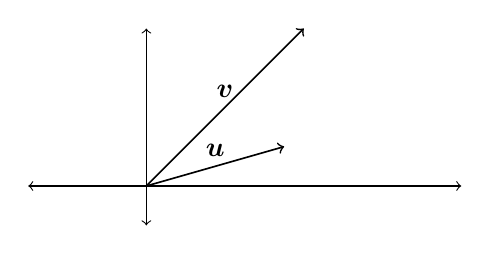
\begin{tikzpicture}
%				\begin{axis}[axis lines=center, xmin=-5,xmax=5,ymin=-5,ymax=5, xticklabel=\empty, yticklabel=\empty, xlabel=\(x_1\), ylabel=\(x_2\), 
%						  ticks=none]
%					
%				\end{axis}
				\draw [<->] (0, -0.5) -- (0, 2);
				\draw [<->] (-1.5, 0) -- (4, 0);

				\draw[->, semithick] (0, 0) -- (1.75, 0.5) node [midway, above] {\(\vec{u}\)};
				\draw[->, semithick] (0, 0) -- (2, 2) node [midway, above] {\(\vec{v}\)};
			\end{tikzpicture}
		\end{figure}
	\end{newquestion}

\fancyhead[C]{\textit{Solutions}}
\section{\centering Solutions}

\subsection{Solutions to \textit{Question 1}}
	\begin{table}[!h]
		\centering
		\begin{tabular}{c@{\hspace{2.5em}}cp{0.75\textwidth}}
			true & false & \\
			\specialrule{\lightrulewidth}{0.25em}{1.25em}
			\bubble & \dbubble & For any scalar \(c \in \mathbb{R}\) and vector \(\vec{v} \in \mathbb{R}^n\), \(\|c\vec{v}\| = c\|\vec{v}\|\). \\[0.75em]
			\dbubble & \bubble & If \(\vec{u} \cdot \vec{v} = 0\), then \(\|\vec{v} - \vec{u}\| = \|\vec{v} + \vec{u}\|.\)\\[0.75em]
			\bubble & \dbubble & If \(\vec{y} \in \mathbb{R}^n\) is orthogonal to some \(\vec{z} \in W\), 
						      where \(W\) is a subspace of \(\mathbb{R}^n\), then \(\vec{y} \in W^\perp\). \\[0.75em]
			\dbubble & \bubble & If \(A \in \mathbb{R}^{10 \times 12}\) and \(\rank A = 6\), then \(\dim (\nullspace A^T) = 6\).\\[0.75em]
			\dbubble & \bubble & If \(\vec{u} \in \mathbb{R}^3\) is orthogonal to \(\vec{w}, \vec{z} \in \mathbb{R}^3\), then
						     it is also orthogonal to any vector in \(\vspan \{\vec{w}, \vec{z}\}\).\\[0.75em]
			\dbubble & \bubble & If \(\dim((\colspace A)^\perp) = 0\) with \(A \in \mathbb{R}^{m \times n}\), then the linear mapping 
						      \(T \colon \mathbb{R}^n \to \mathbb{R}^m\) defined by \(\vec{x} \mapsto A\vec{x}\) is onto.\\[0.75em]
			\bottomrule
		\end{tabular}
	\end{table}

\subsection{Solutions to \textit{Question 2}}
	\begin{table}[!h]
		\centering
		\begin{tabular}{c@{\hspace{2.5em}}cp{0.75\textwidth}}
			possible & impossible & \\
			\specialrule{\lightrulewidth}{0.25em}{1.25em}
			\bubble & \dbubble & 2 planes in \(\mathbb{R}^3\) that are orthogonal complements of each other. \\[0.75em]
			\dbubble & \bubble & Two vectors that form a linearly dependent set but also an orthogonal set. \\[0.75em]
			\bubble & \dbubble & \(A\) is an orthogonal matrix and \(B\) is an orthogonal matrix as well, but \(AB\) isn't. \\[0.75em]
			\bubble & \dbubble & A nonzero vector \(\vec{v}\) with such that \(\vec{v} \in W\) and \(\vec{v} \in W^\perp\). \\[0.75em]
			\bottomrule
		\end{tabular}
	\end{table}

\subsection{Solution to \textit{Question 3}}
	\begin{enumerate}
		\item \textbf{3}. A picture.
		\begin{figure}[!h]
			\centering
			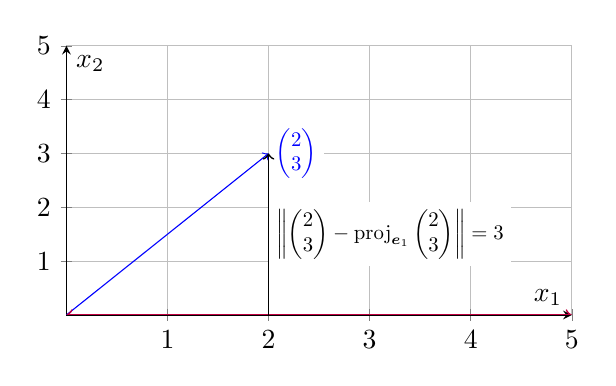
\begin{tikzpicture}
				\begin{axis}[height = 5cm, width=8cm, axis lines = middle, xlabel = {\(x_1\)}, ylabel = {\(x_2\)}, xtick distance = 1, ytick distance = 1, xmin=0, xmax=5, ymin=0, ymax=5, grid=major]
					\plot[blue, ->]coordinates {(0, 0) (2, 3)} node[right, fill=white, scale=0.75] {\(\begin{pmatrix}2 \\ 3\end{pmatrix}\)};
					\plot[<->, semithick, purple, domain=0:5] ({x}, {0});
					\draw[semithick, ->] (axis cs: 2, 0) -- node[right, fill=white, scale=0.75] {\(\biggl\|\begin{pmatrix}2 \\ 3\end{pmatrix} - \operatorname{proj}_{\vec{e}_1} \begin{pmatrix}2 \\ 3\end{pmatrix}\biggr\| = 3\)} (axis cs: 2, 3) ;
				\end{axis}
			\end{tikzpicture}
		\end{figure}
		\item \(\mathbf{\sqrt{10}}\). Another picture.
		\begin{figure}[!t]
			\centering
			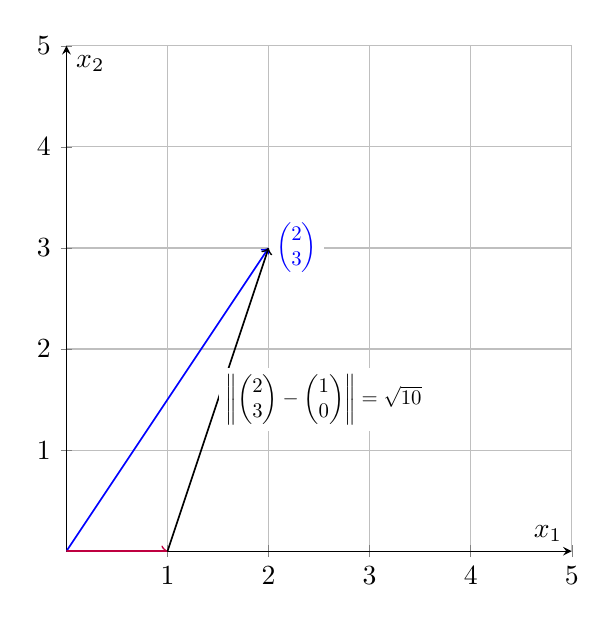
\begin{tikzpicture}
				\begin{axis}[height = 8cm, width=8cm, axis lines = middle, xlabel = {\(x_1\)}, ylabel = {\(x_2\)}, xtick distance = 1, ytick distance = 1, xmin=0, xmax=5, ymin=0, ymax=5, grid=major]
					\plot[blue, ->, semithick]coordinates {(0, 0) (2, 3)} node[right, fill=white, scale=0.75] {\(\begin{pmatrix}2 \\ 3\end{pmatrix}\)};
					\plot[purple, ->, semithick] coordinates {(0, 0) (1, 0)};
					\draw[black, ->, semithick] (axis cs: 1, 0) -- node[right, fill=white, scale=0.75] {\(\biggl\|\begin{pmatrix}2 \\ 3\end{pmatrix} - \begin{pmatrix}1 \\ 0\end{pmatrix}\biggr\| = \sqrt{10}\)} (axis cs: 2, 3);
				\end{axis}
			\end{tikzpicture}
		\end{figure}
	\end{enumerate}

\subsection{Solutions to \textit{Question 4}}
Recall that the coordinates of a vector in the subspace \(W\) are easy to find if we have an orthogonal basis for \(W\). Let 
\(\mathcal{B} = \{\vec{u}_1, \vec{u}_2, \dots, \vec{u}_p\}\) be an orthogonal basis of our subspace. Then, for any vector \(\vec{y} \in W\), we have that 
\[\vec{y} = c_1\vec{u}_1 + c_2\vec{u}_2 + \dots + c_p\vec{u}_p, \quad c_i = \frac{\vec{y} \cdot \vec{u}_i}{\vec{u}_i\cdot \vec{u}_i},\] for \(i = 1, \dots, p\).

In this case, we see that \[[\vec{v}]_\mathcal{B} = \begin{bmatrix}1/4 \\ 1/9 \\ 3\end{bmatrix}.\]

\subsection{Soltuins to \textit{Question 5}}

		\begin{figure}[H]
			\centering
			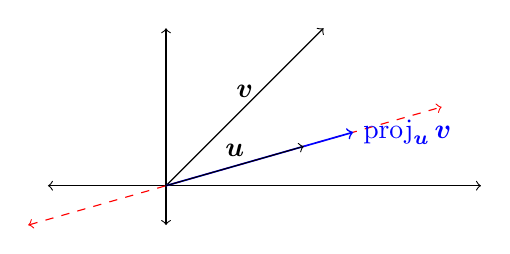
\begin{tikzpicture}
%				\begin{axis}[axis lines=center, xmin=-5,xmax=5,ymin=-5,ymax=5, xticklabel=\empty, yticklabel=\empty, xlabel=\(x_1\), ylabel=\(x_2\), 
%						  ticks=none]
%					
%				\end{axis}
				\draw [<->] (0, -0.5) -- (0, 2);
				\draw [<->] (-1.5, 0) -- (4, 0);

				\draw[->] (0, 0) -- (2, 2) node [midway, above] {\(\vec{v}\)};

				\draw[<->, red, dashed] (-1.75, -0.5) -- (3.5, 1);
				\draw[->, semithick, blue] (0, 0) -- (2.3774, 0.6792) node[right] {\(\proj_{\vec{u}}\vec{v}\)};

				\draw[->] (0, 0) -- (1.75, 0.5) node [midway, above] {\(\vec{u}\)};
			\end{tikzpicture}
		\end{figure}

\end{document}
